%%% The parameter to the ``documentclass'' command is very important.
%%% - use ``review'' for content submitted for review.
%%% - use ``preprint'' for accepted content you are making available.
%%% - use ``tog'' for technical papers accepted to the TOG journal and
%%%   for presentation at the SIGGRAPH or SIGGRAPH Asia conference.
%%% - use ``conference'' for final content accepted to a sponsored event
%%%   (hint: If you don't know, you should use ``conference.'')

\documentclass[tog]{acmsiggraph}

\usepackage{amssymb}
\usepackage{amsmath}
\usepackage[utf8]{inputenc}
\usepackage[table]{xcolor}
\usepackage[colorinlistoftodos]{todonotes}

\setlength{\arrayrulewidth}{1mm}
\setlength{\tabcolsep}{18pt}
\renewcommand{\arraystretch}{2.5}

%%% Used by the ``review'' variation; the online ID will be printed on 
%%% every page of the content.
% \TOGonlineid{12345}

%%% Used by the ``preprint'' variation.
% \TOGvolume{0}
% \TOGnumber{0}

\title{From Particles to Bipeds: Towards More Complex Agent Representations for Crowd Simulations}

\author{Jeff Ames, Benjamin Bancala, Sriharsha Bodapati, Zachary Daniels, \\
        Bhuvana Chandra Inampudi, Le Liu, Renish Matta, Neil Murray, Kevin Shu, Harry Stern\thanks{
          \{jca105, bdb73, sb1129, zad7, bi34, leliu, rm934, npm38, ks788, hcstern\}@rutgers.edu} \\
        Department of Computer Science, Rutgers University}

\pdfauthor{Jeff Ames}

\keywords{STAR, Graphics}

\begin{document}

%\teaser{
%  \includegraphics[height=1.5in]{images/TODO}
%   \caption{TODO}
%}

\maketitle

\begin{abstract}
Agent modeling is a crucial part of crowd simulations. The question arises: what level of realism is appropriate for modeling agents in various situations. In this paper, we survey the existing literature on crowd simulation and show how models can be analyzed by decomposing them along the following three axes: physical representation, mental model and deliberation, and group behavior. This allows us to construct a three-dimensional space in which to categorize existing simulation methods, and suggests a ``holy grail'' of crowd simulations, where realism along all three axes is maximized.
\end{abstract}

\begin{CRcatlist}
  \CRcat{I.3.3}{Computer Graphics}{STAR Topic}{CRcat index}
  \CRcat{I.3.7}{Computer Graphics}{STAR Topic}{CRcat index};
\end{CRcatlist}

\keywordlist

%% Required for all content.
%\copyrightspace

\section{Introduction}

% Problem statement : what is the problem that this research field is tackling ?
Large-scale crowd simulations have traditionally been limited to very simple agent models for reasons of computational efficiency. For example, agents may be a simple disc with position, velocity, and some radius for purposes of collision detection. However, modern systems offer enough power to make more complicated models feasible for reasonably large simulations (on the order of 100,000 agents). The question then becomes what level of fidelity is required in an agent model to effectively capture all the dynamics of interest for the simulation.

% Motivation : why is the problem interesting to the community ?
While simple particle-based models are fast and efficient to compute, there are many interesting behaviors that cannot be represented in such a model. For example, humans are wider shoulder-to-shoulder than they are front-to-back, so turning to the side allows them to fit through narrower spaces. Relatedly, this information is also helpful for planning configurations of walking patterns: incorporating the dimensions and constraints of bipedal agents allow for configurations that allow more agents to pass through a wide space when compared to configurations involving those same agents walking side-by-side. This has many implications for the design of public spaces, event halls, and such.

% Example use case : Give a motivating real world application where this research may be put to use and how it can potentially change the world
Consider architects designing a venue for large events. They have to consider how crowds will flow through the building, especially during time-critical events like an evacuation. More realistic models give them a better picture of what constitutes a safe design and allows them to consider different constraints. For example, models have shown that sometimes adding an obstacle to a space actually increases agent throughput by creating a more efficient flow \cite{helbing2002simulation}.

% Application : What are the different applications to the solution of this problem ?
% - What is the spectrum of applications
% - Industrial / Commercial Applications
% - Research / Academic Applications
Agent modeling also has many implications for fields like robotics, where each agent has to act autonomously but also be able to predict the actions of other agents. For example, a humanoid robot designed to assist people at home not only needs to avoid running into static obstacles like walls and tables but also the people, pets, and other robots around them. To do this, these agents need complex representations of themselves and other agents, not only in terms of their body, but also their goals, psychological state, and likely future behaviors.

This question prompts many possible research topics. What is the appropriate trade-off between representation and efficiency? Some tasks may require only a coarse model for accurate prediction (e.g., treating cars as rectangles for traffic analysis) where others require a much higher level of detail. Do all agents in the scene need to be treated similarly? When can a group of individuals be approximated by a single agent? In some cases, such as with autonomous robots, there may be limitations placed on power usage that affect the computational power available. In such a case, what is the best strategy to maximize predictive power without expending too much energy?

% Requirements / Features: What are the different requirements (identify axes)
To classify existing approaches to these problems, we classify solutions along a few dimensions. First, we look at the physical representation they choose. This ranges from simple disc-like models, as mentioned above, to bipeds like those used in animation rigs, to highly complex biologically-realistic humanoid models, which include bio-mechanical details like human musculature.

Secondly, we examine how the model treats the mental state of the agent. Simple models like ragdolls are oblivious to their environment and are entirely passive. More complicated models respond to stimuli, try to predict the actions of other agents around them, plan for the future, and at the extreme, model complicated human thought processes even at the level of models of realistic neural systems.

Finally, we consider how the model treats 
of individuals. Na\"ive models may treat every individual separately, but more realistic models consider interactions between individuals. For example, birds form flocks in specific patterns when flying. % TODO: \cite{}
In addition to considering agents as individuals, more complex models would include notions of families, group, and societies.

% Challenges : What are the different challenges towards addressing each of these requirements ?
The challenge with each of these refinements is that they make simulation more complex, especially when dealing with thousands of agents simultaneously. For more realistic physical simulation, there are many more degrees of freedom, which makes path planning, animation, and collision detection much more costly. With better mental models come higher cost in prediction, path planning, and error correction when predictions go awry. Modeling groups as well as individuals adds a hierarchy of complexity, with separate factors acting at each level.

% Holy grail : What is the holy grail of this solution ?
In the ideal case, we could model a large group of biologically realistic humanoid agents who would look and act like real people. They would form and dissolve groups on an ad-hoc basis, move realistically, and appear to experience real emotions (panic in case of evacuation, hesitation about which fork in the road to take, etc.). While this may not be feasible for the foreseeable future, we can currently try to find a trade-off within each of the three previously mentioned areas to develop an efficient simulation that still produces interesting results.

% Prior Work : What are the different ways people have approached this problem ? Identify the spectrum / axes of the work ?
% - Create taxonomy, identify categories
% - Industry / Commercial tools : What is the industry currently using ?
% - Research / Academia : What is the current frontier in academic research ?
% - Explain discrepancy between industry and academia, if any
\begin{table*}
\centering
\begin{tabular}{|l|l|l|} \hline
Body                      & Mind                & Group      \\ \hline
particles                 & passive             & individual \\
biped walking             & reactive            & family     \\
footsteps                 & prediction          & group      \\
autonomous robotics       & planning            & society    \\
generalized biped walking & space-time planning & crowd      \\
human biomechanics        & learning/memory     &            \\
                          & artificial life     &            \\ \hline
\end{tabular}
\caption{Stages in model classification}
\label{table:axes}
\end{table*}

More specifically, we break our three axes of classification into the stages listed in Table \ref{table:axes} (where ``body'' denotes a realistic body representation, ``mind'' denotes a realistic model of deliberation, and ``group'' denotes group vs. individual behavior).

% TODO: industry
% TODO: academia
% TODO: discrepancy

% Evaluation : How is this area of research evaluated ? (quantitative, qualitative)
% - Identify axes of evaluation

Research in agent simulation studies is difficult to evaluate quantitatively. There are many aspects of data to analyze which lead some tests to run better than others based on varying optimization. Generally a framework is used to evaluate simulation algorithms and crowd movement. General quantitative parameters would be efficiency and the time complexity of the model. Benchmarks can be used to obtain analyses of shortest path and least collisions. Furthermore, the modeling of the agent is commonly evaluated by the gait of the agent. While evaluating group behaviors, the time to reach the goal, number of collisions and the energy of the system are taken as the benchmark parameters. Qualitatively, a fluid or dynamic movement that more closely resembles biped motion would be ideal when observing simulations side by side. Qualitative analysis is more readily evaluated.

% Each axes of classification listed above can be evaluated separately... 

% Because parameters can be changed to suit different situations, ...
% Axes:
	% how it appears
    % efficiency
    % time complexity 
% Quantitatively: benchmarks for shortest path/ quickest route, least collisions
% Qualitatively: Observably more fluid/realistic (human like) movement when simulations are run side by side

% Benefits and trade-offs : What are the different benefits and trade-offs?
% Stumbled on this source: http://www.cs.uu.nl/docs/vakken/mpp/papers/21.pdf

We now consider the benefits and trade-offs one faces as complexity in physical modeling, behavioral modeling, and crowd modeling increase.

\subsection{Increasingly Complex Physical Models}

First consider simple particle systems. Such a system is good for studying crowd behavior where the motion of the agents is more important the physical properties of the agents. Simple particle systems require less memory than more complex representations because each agent is only required to store its position and motion-related properties such as velocity and acceleration. These systems also tend to be less computationally expensive because they don't need to account for realistic rendering or physics. As we increase the complexity of the agent representation, we can begin to study more interesting behaviors. We can see what actions an agent is physically capable of making and can model more complex situations such as the ``turning sideways'' example previously mentioned. Likewise, we can begin to reduce the search space by pruning states based on impossible physical movements. However, the computational expense will likely increase as the complexity of the agent representation grows because rendering becomes more realistic and the state space might increase because increased realism means agents are no longer bound to a small set of simple actions, and we must begin accounting for interactions with physically-realistic environments and other physically realistic agents. Lastly, the memory required for more complex agents will grow dramatically.

\subsection{Increasingly Complex Behavioral Models}

Consider modeling the behavioral interactions between agents. At the simplest level, the agents do not interact at all. This has the benefit of being computationally efficient: the agent plans thinking of itself. At the next level, the agent becomes aware of other agents, but they still plan individually. Computational cost increases because now the agent has to try to predict how the other agent will move, vastly increasing the search space. If instead, each agent takes a reactive approach, the agents will no longer be able to find optimal paths. At the next level, agents begin cooperating with one another. This might help reduce computational cost because the burden of figuring out the best sequence of actions to take is shared between agents, and the likelihood of collisions decrease because each agent knows the actions the other agents will take. At the next level, we introduce social group behavior between agents, computational costs decrease because now we can treat groups of agents as one entity, but it becomes harder to model complex interactions between groups of realistic agents. Though representing group of agents as an entity decreases the complexity of the search space, the ``human-like'' interaction would be lost as there won't be any individual traits for an agent. A hierarchical structure would work best, but that would again increase the complexity of the model.

We should also consider modeling the psychology of agent models. At the lowest level, agents have no intelligence and act according only to the ``rules'' they are programmed to follow. This means they exhibit very predictable, easily explained behavior, and computational costs are low. As we add more human-like intelligence, agents become more realistic which allows us to better understand human behavior. We can also model more complex and realistic situations. However, this comes at a cost: much less predictability and potentially models that are too complex for humans to interpret. Perfectly modeling an agent as a human would involve introducing things such as emotions and irregularities in behavior, and these would lead to behaviors that are close to impossible to predict. Likewise, modeling such human-level intelligence would require incredible computational resources and likely unfathomable complexity in the representation (e.g. modeling the entire human brain computationally).

\subsection{Increasingly Complex Group Models}
We touched upon this in the previous section: increasing the behavioral complexity of groups would result in simulations that allow for more interesting analysis, but at the cost of increased computational resource use. Alternatively, we can increase the complexity of crowds by increasing their sizes and introducing complexity to the agents' environments. Once again, we can better simulate human behavior but at the cost of increased computational complexity. To address this, one must start modeling the behaviors of groups of agents, but modeling such behavior isn't incredibly well understood yet, and the models might end up being less interpretable than those for individual agents.

% Open Problems : What are still some of the open problems that need to be addressed by this community ?
The major problem that will always linger in the community is the actual mapping of a particle to a biped. As explained above, bipeds are much more complex than particles. Trying to produce a particle that can behave like a biped or even shares some of the major characteristics becomes an extremely expensive operation. The more complex we try to make these particles, the more computational resources are required. This leaves the question, which of these characteristics are trivial and which can we simply ignore? Adding too many characteristics leaves us with great data, but we lose the fast data that we would obtain with a very primitive particle. Removing too many characteristics leaves us with much less data and a simulation that does not accurately represent biped behavior. How do we find the right balance? This would obviously have to be handled on a case by case basis because sometimes speed takes a priority to detail and vice-versa. The community is always looking for new and efficient ways to add more to particles without losing the very reason we model with particles in the first place. 

% Future Work : Forecast the future of this research area

As computational power increases, the demand on resources will lessen and it will be more reasonable to represent perfectly human simulations all the time. Eventually it may be pointless to abstract from particles to bipeds at all. The physical constraints will most likely be the first problem solved with future research. Group interaction and realistic thinking may never find a perfect solution because they may be ever changing. The methods to evaluating these constraints however will most likely become more efficient, and implementations may be trivial.

\section{Feature matrix}

\begin{table*}[t]
\begin{tabular}{|l|c|c|c|} \hline
Solution & Physical Constraints & Realistic Thinking & Group Interaction \\ \hline
Footstep Navigation & \checkmark & X & X\\
Individual Agent Control & \checkmark & X & X \\
Human Behavior Models & X & \checkmark & X\\
Cooperative Collision Avoidance & X & \checkmark & \checkmark \\
Social Group Behavior Models & X & \checkmark & \checkmark \\ \hline
``Holy Grail'' & \checkmark & \checkmark & \checkmark \\ \hline
\end{tabular}
\caption{Feature Matrix for Various Approaches Proposed in the Literature}
\label{table:feature-matrix}
\end{table*}

In Table \ref{table:feature-matrix}, we propose a matrix that attempts to group various approaches in the literature by the constraints addressed in their models. The column ``physical constraints'' denotes a realistic physical representation; in some cases this means modeling the whole human body while in others it means modeling specific physical traits of biped motion. ``Realistic thinking'' denotes models that utilize a realistic model of deliberation or some human-like `psychological' behavior. ``Group interaction'' denotes attempting to model groups as larger entities instead of interactions between individual agents. We plot each approach relative to one another along the three previously defined categories of complexity in Figure \ref{fig:fs}.

\begin{figure}[ht]
\centering
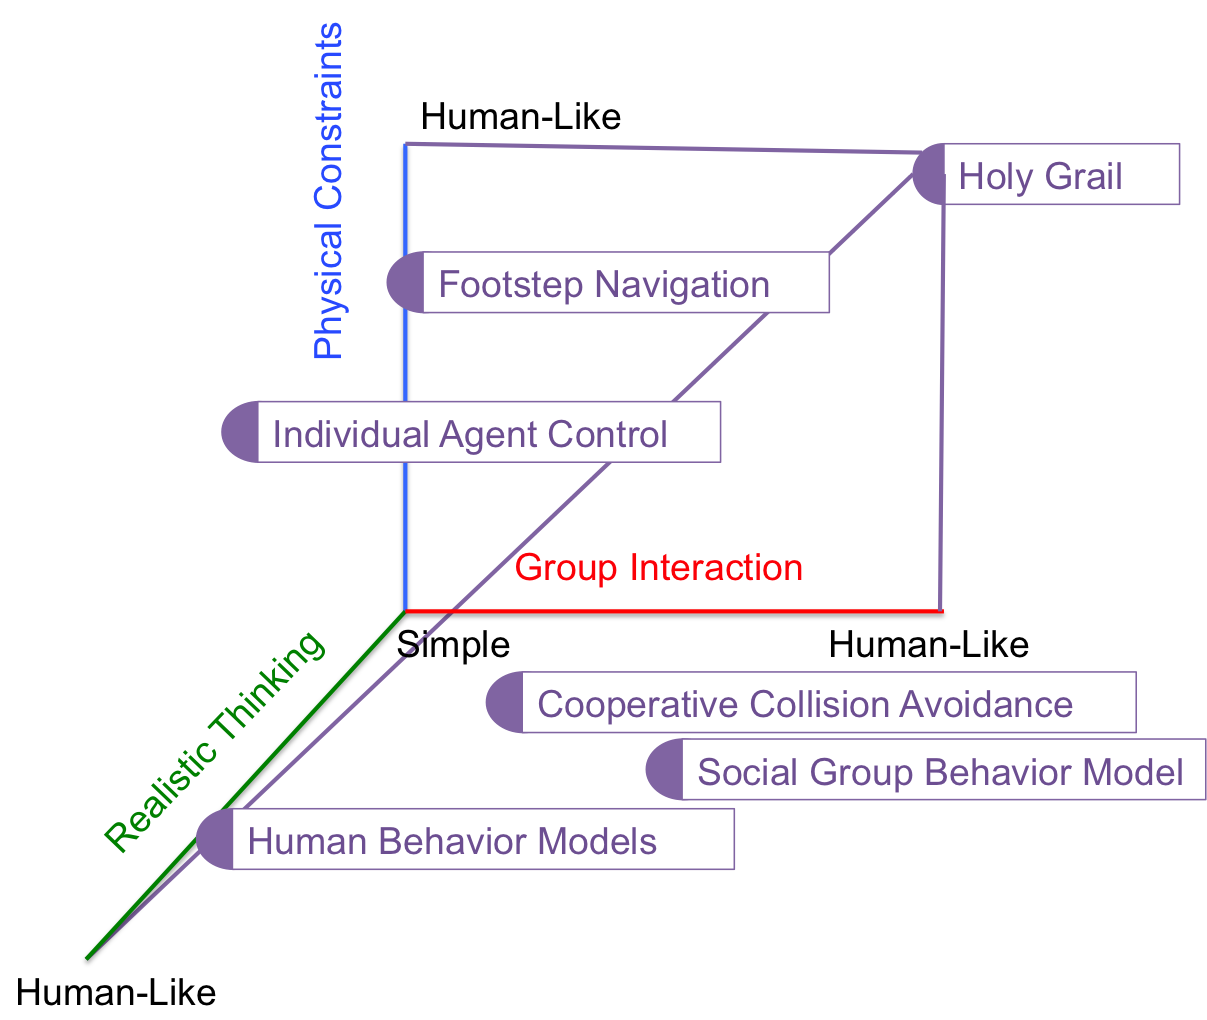
\includegraphics[width=.50\textwidth]{images/FeatureSpace.png}
\caption{We plot where each approach falls in a 3-dimensional feature space}
  \label{fig:fs}
\end{figure}

\section{Background}

An area of recent interest is analyzing behaviors and movement in crowds. Very often the agents of greatest interest in crowd analysis are real-life entities such as human beings, birds, and robots. Such agents often have many intricacies and physical constraints that make realistic modeling by computer simulation very difficult. In order to reduce complexity in such problems, these entities are often represented as simple particles, and such a simplification typically helps those studying crowd analysis discover general trends in group and individual behavior and movement. An adverse effect to modeling agents as particles is that there is a loss of information and realism that limits the types of problems that can be studied by crowd simulation. We aim to investigate several key issues:
\begin{enumerate}
\item How can we go from modeling individual agents as particles to more complex entities (typically bipeds)?
\item What physical constraints are important to model at an agent-level?
\item What trade-offs between realism and computational/representational complexity must be made when modeling complex agents?
\item What types of problems can be studied once we have more complex representations of agents?
\end{enumerate}

We broadly divide related work into the following categories, which are described in more detail below: agent-based steering in crowds, obstacles and collision avoidance, and group behaviors.

\subsection{Physical representation}

In the first section of this paper, we examine several papers concerned with designing steering algorithms for individual agents. These algorithms focus on three general aspects of steering: i.) incorporating physically realistic constraints ii.) integrating step placement iii.) introducing human-like behaviors and action sequences.

\subsection{Mental model and deliberation}

Collision avoidance for a single particle-like agent has its challenges, but these are compounded when we move to a multi-agent system with more realistic agent models. In particular, agents need some mental state to estimate other agents' future positions, goal points, and intended paths. In this section, we explore how realistic rendering of agents affects algorithms for collision avoidance and dealing with obstacles.

\subsection{Group behavior}

In a previous section, we investigated how making agents more complex affect behavior at the individual, agent-based level. In this section, we explore how adding additional physical and behavioral constraints affect crowds at a group-level. We see common trends in the types of questions asked, e.g. what physical and behavioral constraints must be added, and how do these constraints shape the algorithms for simulating and analyzing crowds? Specifically, the papers mentioned in this section largely focus on how complex agents interact at different levels of a crowd ``hierarchy'': small groups, larger `flocks', and the crowd as a whole and how the behavior and walking patterns of individual agents shape the crowd behavior as a whole. Questions about how to make crowd simulations more realistic while still being computationally efficient are also addressed.

%\subsection{Agent-based steering in crowds}

% \begin{itemize}
% \item ``Robust Space-Time Footsteps for Agent-Based Steering'' \cite{bersethrobust}
% \item ``Modeling Individual Behaviors in Crowd Simulation'' \cite{braunmodeling2003}
% \item ``On the interface between steering and animation for autonomous characters'' \cite{singh2010interface}
% \item ``Footstep navigation for dynamic crowds'' \cite{singh2011footstep}
% \item ``Controlling individual agents in high-density crowd simulation'' \cite{pelechano2007controlling}
% \item ``Responsive biped character stepping: When push comes to shove'' \cite{kenwright2012responsive}
% \item ``Autonomous pedestrians'' \cite{shao2005autonomous}
% \item ``Adaptive pedestrian behavior for the preservation of group cohesion'' \cite{vizzari2013adaptiveped}
% \item ``Steering behaviors for autonomous characters'' \cite{reynoldssteer1999}
% \item ``Leveraging human behavior models to predict paths in indoor environments'' \cite{tastansuk2011}
% \item ``Exploiting human steering models for path prediction'' \cite{tastansuk2009}
% \item ``A synthetic-vision based steering approach for crowd simulation'' \cite{hal2010}
% \item ``Teaching Bayesian behaviours to video game characters'' \cite{lehy2004teaching}
% \item ``Animation of Human Walking in Virtual Environments'' \cite{chung2000interactively}
% \item ``Synthesis of Constrained Walking Skills'' \cite{coros2008synthesis}
% \item ``Generalized biped walking control'' \cite{coros2010generalized}
% \item ``Virtual Crowds: Methods, Simulation, and Control'' \cite{pelechano2008virtual}
% \item ``Navigation and steering for autonomous virtual humans'' \cite{kapadia2013navigation}
% \item ``Animation of Humanlike Characters: Dynamic Motion Filtering with a Physically Plausible Contact Model'' \cite{pollard2001animationof}
% \item ``From Footprints to Animation'' \cite{panne97footprints}
% \item ``Simbicon: Simple biped locomotion control'' \cite{yin2007simbicon}
% \end{itemize}

% \subsection{Obstacles and collision avoidance}

% \begin{itemize}
% \item ``Reciprocal velocity obstacles for real-time multi-agent navigation'' \cite{van2008reciprocal}
% \item ``Reciprocal collision avoidance with acceleration-velocity obstacles'' \cite{van2011reciprocal1}
% \item ``Reciprocal $n$-body collision avoidance'' \cite{van2011reciprocal2}
% \item ``Generalized velocity obstacles'' \cite{wilkie2009generalized}
% \item ``ClearPath: Highly Parallel Collision Avoidance for Multi-Agent Simulation'' \cite{stephen2009clearpath}
% \item ``A collision avoidance behavior model for crowd simulation based on psychological findings'' \cite{park2013psych}
% \item ``Autonomous mobile robot dynamic motion planning using hybrid fuzzy potential field'' \cite{jaradat2012autonomous}
% \item ``Collision avoidance method for multiple autonomous mobile agents by implicit cooperation'' \cite{abe2001collision}
% \end{itemize}

% \subsection{Group behaviors}

% \begin{itemize}
% \item ``Group Behaviors for Systems with Significant Dynamics'' \cite{brogangroup1996}
% \item ``Crowd and Group Simulation with Levels of Detail for Geometry, Motion and Behaviour.'' \cite{Sullivancrowd2002}
% \item ``Hierarchical Model for Real Time Simulation of Virtual Human Crowds'' \cite{MusseHierarchial2001}
% \item ``Scalable behaviors for crowd simulation'' \cite{sung2004scalable}
% \item ``Simulating the local behaviour of small pedestrian groups'' \cite{karamouzas2010simulating}
% \item ``The Walking Behaviour of Pedestrian Social Groups and Its Impact on Crowd Dynamics'' \cite{Moussaid2010}
% \item ``Animation of Flocks and Herds'' \cite{dadova2010flocks}
% \item ``Emergent behavior in flocks'' \cite{cucker2007emergent}
% \item ``Flocks, herds, and schools: A distributed behavior model'' \cite{reynoldssteer1987}
% \item ``An agent-based crowd behaviour model for real time crowd behaviour simulation'' \cite{kountouriotis2014agent}
% \item ``Intuitive crowd behavior in dense urban environments using local laws'' \cite{Loscos2003reciprocal1}
% \item ``Multilevel model of the 3D virtual environment for crowd simulation in buildings'' \cite{galland2014}
% \item ``Increasing efficiency of crowd simulation using particle swarm optimization'' \cite{kaurrani2013}
% \item ``Crowd simulation incorporating agent psychological models'' \cite{pelechano2005}
% \item ``Simulation of pedestrian crowds in normal and evacuation situations'' \cite{helbing2002simulation}
% \end{itemize}

\section{State of the Art}

\subsection{Physical representation}
Most of the crowd steering algorithms generate force vectors, velocity vectors, center-of-mass trajectories, or discrete behavior actions as their output. This output is then used to produce animation using motion synthesis. In a majority of the cases, a character is represented as an oriented particle that moves by the output generated by the steering algorithms. There are two main disadvantages to this approach \cite{singh2010interface}:
\begin{itemize}
\item \textit{Limited locomotion constraints:} Most of the steering algorithms do not account for locomotion constraints. Trajectories may have discontinuous velocities, oscillations, awkward orientations, or may try to move a character during the wrong animation state, and these side-effects make it harder to animate the character intelligently. For example, a character rarely step backwards for more than two steps at a steady walking speed, while facing forward, and a character moving forward cannot easily shift momentum to the left when stepping with the left foot.
\item \textit{Limited navigation control:} Most of the algorithms assume that an animation system will know how to interpret a vector based steering decision. But a vector does not have enough information to indicate appropriate maneuvers, such as side-stepping versus reorienting the torso, stepping backwards versus turning around, planting a foot to change momentum quickly, or carefully placing steps in exact locations. It is required for steering algorithms to have better control to improve the character’s steering intelligence.
\end{itemize}

\subsubsection{Footstep model}
The footstep model focuses on generating footsteps as the output. A well-constrainted footstep model will address the above challanges as footsteps are an abstraction for most locomotion tasks and they provide precise, unambiguous spatial and timing information to animation.
\\
\cite{singh2011footstep} defined a system in which each step is derived by a 2D parabolic trajectory that approximates the motion of a 3D inverted pendulum. The location, orientation, and timing of footsteps are derived from those trajectories. Additionally, best-first search is used to plan a sequence of footsteps that avoids collisions, satisfies footstep constraints for natural locomotion, and minimizes the effort to reach a local goal. 
\\
This model's basis is formulated based on the analogy between human locomotion and the inverted pendulum i.e., the pendulum pivot represents a point on or near a footstep, while the pendulum mass represents a character’s center of mass. The dynamics of an inverted spherical pendulum are approximated using parabolas. Piecewise parabolic curves are enough to capture the variety of trajectories that a human’s center of mass will have: varying curvature, speed, and step sizes.
\\
First, the orientation of the parabola is used to compute a transform from world space to local parabola space. Then, the direction of velocity from the end of the previous step is transformed into local space, normalized, and re-scaled by the desired speed. With this local desired velocity, there is enough information to get the parabola to be approximated. And then, the next step is calculated based on the parabolic equation. The formulation of foot step model can be seen in figure \ref{fig:FootSetp}.

\begin{figure}[h]
  \begin{center}
    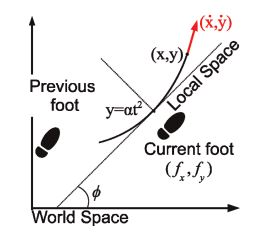
\includegraphics[width=0.48\textwidth]{images/FootStep}
  \end{center}
  \caption{Foot  step model formulation. Image Courtesy of [Singh et al.\ 2011] }
  \label{fig:FootSetp}
\end{figure}
Many properties of human locomotion are automatically enforced by the definition of this model. The piecewise parabola will be G-1 continuous. The center of mass will remain between the two feet by enforcing the local-space parabola remains positive.

% \subsubsection{Model 2}

% Physical representation:
% - particles
% - simbicon
% - footsteps
% - asimo
% - generalized biped walking control
% - human biomechanics

% http://dl.acm.org/citation.cfm?id=1559756
% http://web.cs.ucla.edu/~dt/papers/siggraph06/siggraph06.pdf
%
% look at other work by these authors

\subsection{Mental model and deliberation}

\subsubsection{Deliberation for Collision Avoidance: Velocity Obstacles, Reciprocal Velocity Obstacles, and Related Concepts}
\textbf{i. Basic Formulation}
There is a lot of work on reactive collision avoidance. In this section, we focus on a set of algorithms that do not explicitly communicate with one another, but deliberate by establishing a predetermined policy for how to move in the case of an immanent collision. As such, these agents move beyond simple particles to deliberating particles to deliberating agents with additional kinematic constraints. We first introduce the simplest of these algorithms, the velocity obstacle. We then look at reciprocal velocity obstacles (RVOs) and variants of RVOs as well as other similar algorithms and other extensions and generalizations of velocity obstacles.
\\
Velocity obstacles were originally formulated by Fiorini et al.\ \cite{fiorini1998motion}. Velocity obstacles define the set of potential velocities for an agent and an obstacle that would result in a collision between the agent and obstacle. By selecting a feasible velocity for the agent outside of this set, collisions can be avoided. As such, velocity obstacles are typically used as in reactive algorithms for collision avoidance on top of some global path planning algorithm. Velocity obstacles can be efficiently computed by exploiting the computational geometry of the problem, computation of velocity obstacles are highly parallelizable, and algorithms built on velocity obstacles scale linearly with the number of agents. Because of their low computational cost and ease of implementation/integration into existing global path planning algorithms, velocity obstacles are a popular algorithm for collision avoidance. An illustration of the geometry beyond velocity obstacles can be seen in \ref{fig:vo}.

\begin{figure}[h]
  \begin{center}
    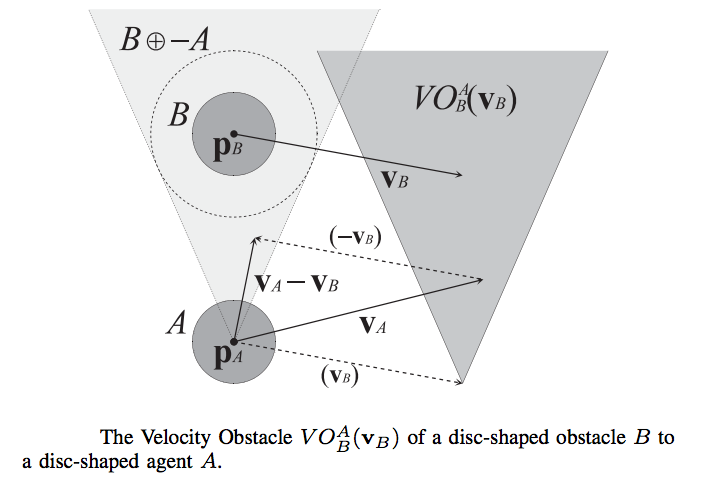
\includegraphics[width=0.48\textwidth]{images/VO}
  \end{center}
  \caption{The geometry of velocity obstacles. Image Courtesy of [Van der Ber et al.\ 2008] }
  \label{fig:vo}
\end{figure}

Velocity obstacles are not without their flaws. In the following sections, we show how velocity obstacles can be generalized and extended to account for additional knowledge and constraints.  
\\ \\
\textbf{ii. Reciprocal Velocity Obstacles (RVOs)}
\\
When using traditional velocity obstacles, we assume that agents act independently of one another (except for having knowledge of each other's position). Algorithms based on reciprocal velocity obstacles pre-establish a policy for how both agents should move when a collision is imminent \cite{van2008reciprocal}. Specifically, when two agents are on a collision path, each agent should choose a new velocity that is the average of the agent’s current velocity and a velocity that lies outside the other agent’s velocity obstacle. This differs from traditional velocity obstacles where each agent selects a new velocity that is completely outside the other agent’s velocity obstacle. When computed between two agents and assuming there is some feasible choice of velocities for which the collision is avoidable, this guarantees a set of actions that will result in collision-free movement, and furthermore, it will guarantee oscillation-free movement. An example of such movement can be seen in \ref{fig:rvo}. This oscillation-free guarantee cannot be made for traditional velocity obstacles. Likewise, all of the same benefits that hold for traditional velocity obstacles, namely computational efficiency, hold for RVOs as well. RVOs are still a reactive and local algorithm, so they will still find suboptimal paths and get stuck in local minima if not used on top of a global path finding algorithm. Additionally, RVOs assume unconstrained motion (i.e.\ instant pivoting and instantaneous change in velocity).

\begin{figure}[h]
  \begin{center}
    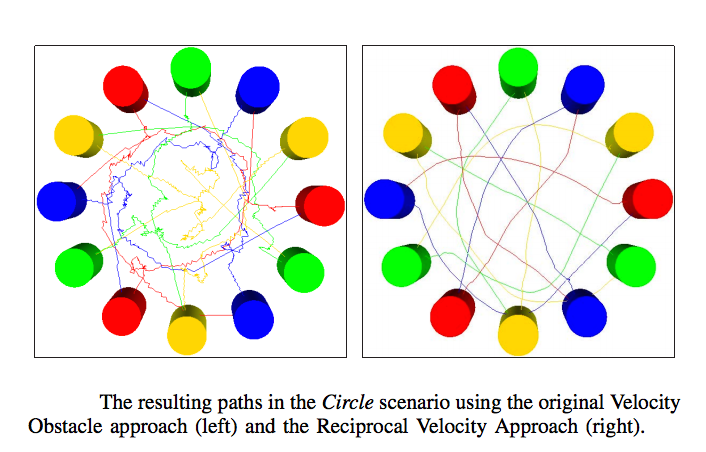
\includegraphics[width=0.48\textwidth]{images/RVO}
  \end{center}
  \caption{A visual example of the difference between avoiding collisions using traditional velocity obstacles and reciprocal velocity obstacles. Note the lack of spiraling and smoother, less oscillatory paths when using RVOs compared to VOs. Image Courtesy of [Van der Ber et al.\ 2008] }
  \label{fig:rvo}
\end{figure}

\textbf{iii. Common Velocity Obstacles (CVOs)}
\\
Common velocity obstacles are extremely similar to RVOs \cite{abe2001collision}. CVOs operate using implicit cooperation. Avoiding collisions involves optimizing trajectories using velocity obstacles. CVOs are plagued by the same problems as RVOs.
\\ \\
\textbf{iv. Generalized Velocity Obstacles (GVOs)}
\\
Velocity obstacles assume that agents move in an unconstrained manner. In practice, this is not a good assumption. For example, consider car-like agents. Such agents cannot instantly adjust direction and speed; they require additional time and space to reach certain states. Wilkie et al.\ expanded velocity obstacles to work with agents with kinematic constraints \cite{wilkie2009generalized}. While GVOs overcome a major problem of velocity obstacles, they fail to address and even add several others. First, they do not use reciprocity, so they are not guaranteed to be oscillation-free. Furthermore, they are only guaranteed to be collision-free under much stronger assumptions than traditional velocity obstacles. The paths produced using GVOs are only piecewise smooth. Lastly, the way in which GVOs are computed can be numerically unstable, and thus, it may be required to place a small safety buffer around each agent resulting in suboptimal movement.
\\ \\
\textbf{v. Acceleration-Velocity Obstacles (AVOs)}
\\
Traditional velocity obstacles and RVOs don't consider constraints on acceleration. These constrations were added in \cite{van2011reciprocal1}. AVOs operated by using proportional control to accelerate agents to a new velocity. Proportional control means the applied acceleration is always proportional to the difference between the new velocity and current velocity. AVOs are formulated for holonomic (physically unconstrained) agents, but assuming non-zero speed, can extended to agents with kinodynamic constraints such as cars, planes, and vehicles using differential drives. AVOs are good for agents moving at high speeds. Once again, AVOs face the same issues related to reactive collision avoidance that the other velocity obstacle-based algorithms face. Likewise, AVOs do not currently generalize to movement in three dimensions.
\\ \\
\textbf{vi. Hybrid Reciprocal Velocity Obstacles (HRVOs)}
\\
Hybrid reciprocal velocity obstacles are very similar to RVOs \cite{snape2011hybrid}. They differ by attempting to avoid the ``reciprocal dance'' whereby two agents waver when trying to pass one another specifically because they take into account a predetermined agreed upon policy. HRVOs solve this problem by enlarging the reciprocal velocity obstacle on the side of an agent that the other agents should not pass.
\\ \\
\textbf{vii. Recursive Probabilistic Velocity Obstacles (RPVOs)}
\\
Recursive probabilistic velocity obstacles extend velocity obstacles in two ways: they introduce the concept of uncertainty to velocity obstacles and they can handle more than two agents at a time \cite{kluge2006recursive}. They attempt to reason about other agent's perception and motion. They introduce uncertainty in both the shape of other agents and the velocity of other agents. However, while RVOs are guaranteed to find collision-free trajectories, RPVOs are not guaranteed to converge to a solution.
\\ \\
\textbf{viii. Optimal Reciprocal Collision Avoidance (ORCA)}
\\
Van der Berg et al.\ propose an alternative method for avoiding collisions between many agents \cite{van2011reciprocal2}. They formulate collision avoidance as a linear program and solve for the new velocities of all participating agents. In this way, they are guaranteed to move optimally and avoid all collisions if such a solution exists.  In this same paper, they also add acceleration constraints to RVOs and propose extensions to their method that would apply to both holonomic and kinematically-constrained (e.g. car-like) agents. However, such extensions make assumptions that might result in sub-optimal movement. Lastly, their method does not generalize to movement in 3-dimensions.

\subsubsection{Mental Models for Collision Avoidance: Collision Avoidance Based on Psychological Phenomena}
RVOs, while interesting, are still fairly simple models for predicting agent movement. One interesting line of work in the collision avoidance literature is to try and mimic how humans avoid colliding with one another. Park et al.\ propose a method for collision avoidance based on psychological observations \cite{park2013psych}. By examining a few key behaviors of humans, collisions can be predicted and avoided without knowing the other agent's exact trajectories. The opposing agent's gaze movement angle (GMA) is used in conjunction with speed-variant Information Process Space (IPS) to predict mid- to long-range collisions. IPS is defined as ``a conceptual area that determines the spatial boundary within which all other pedestrians are treated as potential clashers to the observing pedestrian'' \cite{park2013psych}. Next, side-stepping and gait motion are used to steer the agent, and movement is restricted by an agent's personal reaction bubble (PBR), which is a hierarchy of spaces which affect an agent's comfort level. These are the intimate space, personal space, social space, and public space, and the PBR is often modeled by concentric ellipses. Park and company's method has some very nice advantages over traditional collision avoidance algorithms like RVOs: they are more robust to variations in the speed and path of pedestrians, they are psychologically-grounded, and they better model human-like movement/behavior. Of course there are also flaws. They require agents that exhibit human behaviors such as gaze and different gaits, they are still a local/reactive method for collision avoidance (and thus give sup-optimal movement along the global path), and they have much higher model complexity than traditional approaches to collision avoidance.


% Thinking/deliberation:
% - passive (inanimate / ragdoll)
% - reactive (FSMs, rule-based systems)
% - prediction (predicting other agents' movement in the next time step)
% - planning (planning many steps ahead in a static environment)
% - space-time planning (planning in space-time, including other agents' movements)
% - learning/memory (machine learning models)
% - artificial life and neural models

% ALIFE:
% autonomous pedestrians: http://web.cs.ucla.edu/~dt/papers/gmod07/gmod07.pdf
%
%
% planning:
% http://www.cs.rutgers.edu/~mk1353/projects-mdp.html
%
% predictions:
% http://gamma.cs.unc.edu/ORCA/
% (there are many variants of this -- cite them)
% HRVO
% GVO
% RVO
% etc
%
% learning / memory :
% not much work here -- you will have to dig in other communities

\subsection{Group behavior}

Accurate crowd simulation has been a topic of increasing interest over the years, both for its use in video games and for its application in the study of human behavior in virtual environments. However, it is actually extremely difficult to create realistic crowd simulations due to the computational intensity associated with increasing the level of sophistication of each individual within a crowd so they react realistically to their surrounding. Simulating each individual as a unique agent with complex artificial intelligence consumes too much processing power for current hardware to handle. Fortunately, research has started exploring alternatives that might provide an adequate solution to the problem. Instead of giving each agent complex steering logic, this logic can be externalized to a third party. Since specialized logic is removed from standard agents, less computation is needed and overall performance is enhanced.

One solution is the use of situation agents that allow the basic agents to retain only the most basic form of steering while the situation agents handle the more complex movements. ``Situation agents are similar to standard agents in many regards: they have a defined location, size, velocity, and goal. They can utilize steering strategies to interact with other situation agents. However, they differ from standard agents in that they exist solely to supervise the actions of other agents in localized scenarios that their typical steering algorithms might not support'' \cite{schuerman2010situation}. By employing them, the majority of the agents can maintain just the fundamental steering logic and be guided to move in a certain fashion by the situations agents, which eliminates a large portion of the processing needed. The situation agents also allow for easily scaling to larger simulations since relatively small numbers of them can dictate the behavior of large groups of agents. 

``Situation agents coordinate the behaviors of other agents by modifying those agent’s parameters. In the their most general form they can modify any parameter within any agent, including other situation agents'' \cite{schuerman2010situation}.  Various situation agents can be used to satisfy different steering conditions. All steering frameworks calculate either a best path or best velocity for each agent which will most directly guide them toward their goal during each iteration. Situation agents are able to modify this to herd other agents when required. For situations such as deadlock, basic agents are instructed to yield by ``reducing their boldness and modifying their preferred velocities'' \cite{schuerman2010situation}.  This causes the agents not moving in the favored direction to move aside so others can pass. Situation agents can also direct a group to move as a whole by steering the basic agents to avoid other group agents with different goals and linearly combine the resulting velocity with the preferred velocities of the group’s members. 

Another answer to simplify crowd simulations are composite agents. They work similarly to the situation agents, creating group behavior by directing the basic agents, but they use a different approach. A composite agent is a basic agent that is associated with a set of proxy agents. The behaviors of these proxies are coordinated with that of the basic agent to achieve particular effects. ``A proxy agent includes an external state which consists of the same properties as in the basic agent’s external state, and a unique internal state'' \cite{yeh2008composite}. The fact that a proxy agent possesses the same set of external properties as a basic agent and the fact that the function which update the agents’ state only considers the external states of the neighboring agents leads to the central idea behind composite agents: both the basic agents and proxy agents are treated uniformly by the UPDATE function. Therefore, other agents react to a proxy agent in exactly the same way as they would to a basic agent. The ``proxy agent, however, updates itself according to a unique set of rules, defined in the P-UPDATE function'' \cite{yeh2008composite}, which updates independently based on the behavior the composite agent is trying to promote. This allows the influence that a composite agent exerts over other agents to indirectly include all the influences of its proxy agents through which it is able to affect the behavior of the agents around it. 

In figure \ref{fig:le}, we see how the composite agent(C) uses its proxy agents(P) to affect the behaviors of the basic agent(A).

\begin{figure}[ht]
\centering
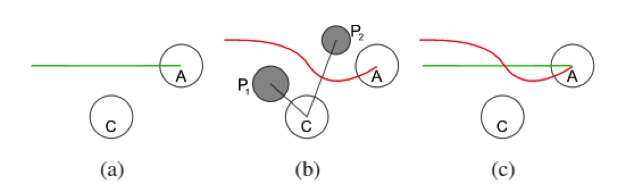
\includegraphics[width=.50\textwidth]{images/leimage.png}
\caption{We see how the composite agent(C) uses its proxy agents(P) to affect the behaviors of the basic agent(A). Image Courtesy of [Yeh et al.\ 2008] }
  \label{fig:le}
\end{figure}

	Crowd observation and crowd representation play a huge role in how people see the simulations. To create crowd movements, ``simulations should exhibit human behaviors for navigation, pedestrian decision making, and social behaviors such as grouping and crowding'' \cite{park2013modeling}. This needs to be understood because the crowd simulations should avoid collisions and path finding should be clear. This results in ``visually pleasing steering behaviors of virtual humans'' when observed \cite{park2013modeling}. There are several approaches to how these crowds can be observed in their simulations and behaviors. 
	
	Groups in a crowd can be modeled for their behaviors and simulations by using multiple agents. This is by using the common ground-based crows simulation (CGCS) model \cite{park2013simulating}. It is defined as ``a model for multi-agent systems using agent-based modeling method. For example, individual agents are capable of perceiving and responding to their immediate surroundings, and are organized into groups or ‘co-travellers’. These group members maintain group cohesiveness by communicating and adapting their behaviors to each other while walking'' \cite{park2013modeling}.
These observed groups are not individual agents that are alone. As Park states, ``up to 70 percent of observed pedestrians are walking in groups, and most groups are composed of a small number of members. These groups that are walking and their behaviors ``should be modeled by taking a perspective of mindful entity as a social group to achieve the enhanced realism in crowd simulations'' \cite{park2013modeling}. 

There are different types of strategies for how crowds and behaviors are represented that show how crowds operate. The first is called Macro–coordination strategies which ``relate to overall action plans to accomplish the groups' goals. So, these strategies are dependent on the domain. For example, one can have a group of soldiers and may select a particular strategy by training and doctrine, while a group of friends at a sporting activity may decide how to meet at a predetermined location'' \cite{park2013modeling}. 

The other strategy is called Micro-coordination and this ``relates to dynamics of human and communicative behavior.'' The specifics of Micro-coordination are that it is ``determined to a degree by the constraints of human perception, the physics of sound in voice communication, and cultural concerns.'' Also, this strategy is "influenced by the state of the immediate environment. For example, the voice communication in a movie theater may be suppressed. Or, visual displays and uptake may be constrained in a dense crowd" \cite{park2013modeling}. Overall, it is a set of actions for group members to get each other to understand what is intended. In figure 4, we see examples of micro behavior.

\begin{figure}
\centering
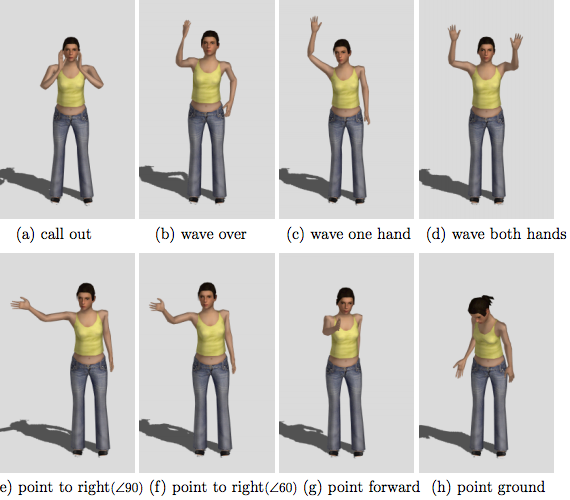
\includegraphics[scale=0.4]{images/parkimage.png}
\caption{We see examples of micro behavior consisting of actions such as call out, wave over, point to right, ...etc that would help understand the communication within groups. Image Courtesy of [Seung In Park.\ 2013] }
  \label{fig:park}
\end{figure}

When simulating agents in groups, it is important to account for different situations in which groups of agents can be found in.  In fact ``one of the least studied and understood aspects of crowds of pedestrians is represented by the implications of the presence of groups'' \cite{vizzari2013adaptiveped}.  In most current models, ``the presence of other individuals as a sort of moving obstacle or simply as openers of a potential route to follow,'' which is not conducive to adaptive behavior \cite{vizzari2013adaptiveped}.  Groups of agents should be able to react adaptively when placed in a situation such as one in which the overall crowd density changes.  Another example would be a situation in which the spatial configurations or the area in which the groups are simulated changes.  The Adaptive pedestrian behavior for the preservation of group cohesion research paper delves into this matter, looking into a agent-based system which is able to adapt to different situations.

This model is dependent on the following factors: representation of the environment, definition of spatial markers and definition of floor fields.

The environment in this model is represented by square cells where each cell has a row and column to indicate its position in a grid.  ``Every cell in the environment can be in three possible states: free, occupied by an obstacle, or occupied by a pedestrian'' \cite{vizzari2013adaptiveped}.

Spatial markers are used to specify what role certain spaces in the environment have in the model.  There are three types of spatial markers: start areas, destination areas and obstacles.  Start areas are the spatial markers where pedestrians are generated.  Destination areas are the final location where the pedestrians need to go.  Obstacles are cells of the environment which are not accessible to the agents.  In other words, the agents cannot move into cells whose spatial marker is set to obstacle.

Floor fields are ``a set of superimposed virtual grids, structurally identical to the environment grid, that contains different floor fields that influence pedestrian behavior. The goal of these grids is to support long range interactions by representing the state of the environment (namely, the presence of pedestrians and their capability to be perceived from nearby cells) in terms of field modifications'' \cite{vizzari2013adaptiveped}.  Three types of floor fields used in this model are: path fields, obstacles fields and density fields.  Path fields determine the distance of every cell from the destination.  Obstacle fields indicates every cell which is an obstacle.  Density fields indicate the pedestrian density in surrounding cells for each cell in the current time-step.

Like in previous models, this model depends on simple groups which are groups ``bound by a strong relationship (e.g. friends, family members): the agents representing members of this kind of group are characterized by an adaptive behavioral mechanism aimed at preserving its cohesion, even in situations of high local density and presence of obstacles or counter flows of other pedestrians'' \cite{vizzari2013adaptiveped}.  This model also depends on structured groups, which are ``artificially defined with the goal of organizing and managing the movement (or some kind of other operation) of a set of pedestrians'' \cite{vizzari2013adaptiveped}.  

To evaluate what action to take for this model, ``every time step, every pedestrian perceives the values of path field, obstacle field and density field for all the cells that are in its neighborhood. On the basis of these values and according to different factors, the agent evaluates the different cells around him, associating an utility value to every cell and selects the action for moving into a specific cell'' \cite{vizzari2013adaptiveped}.  What makes this model different from others is that it takes into account factors such as intergroup cohesion and adaptation mechanisms for group cohesion preservation.  With these factors being utilized, it is seen that ``the model produces results in tune with available evidences from the literature, both from the perspective of pedestrian flows and space utilisation, in scenarios not comprising groups; when groups are present, the model is able to preserve their cohesion even in challenging situations (i.e. high density, presence of a counterflow), and it produces interesting results in high density situations that call for further observations and experiments to gather empirical data'' \cite{vizzari2013adaptiveped}.

\subsection{Holy grail}

% Group behavior:
% - individual:
% - family
% - group
% - society
% - crowd

% flocks : boids (reynolds)
%
% http://www.cs.rutgers.edu/~mk1353/projects-situation-agents.html
% http://gamma.cs.unc.edu/CompAgent/
% http://onlinelibrary.wiley.com/doi/10.1111/j.1467-8659.2009.01404.x/abstract
% (look at their related work to find more pointers)
%
% social science -- cooperation --> you will have to look at literature in behavioral science

This brings us to the question of what is the holy grail of realistic crowd simulation. In the ideal case, we could simulate large numbers of agents, with realistic human-like bodies, who have human-level intelligence and communication, and who fluidly shift from acting individually to acting as groups as the situation demands.

In part, however, this depends on the goals of the simulation. For example, when modeling aircraft boarding, only a certain level of physical realism is required. Even cylinders may be sufficient to get an accurate approximation. Similarly, the required mental model is also relatively simple. However, in the case of modeling a complex choreography of dancers or fighters, a much higher level of physical detail is required. In modeling crowd pathfinding in a crowded corridor, we must capture much more of each agent's mental state, their prediction of others' states, and the forces acting on them socially.

While the ``holy grail'' scenario would require prohibitive amounts of computational power (both in terms of CPU and memory), in practice most simulations can be approximated reasonably well with modern-day hardware given the acceptable trade-offs determined by the simulation's desired output.

\bibliographystyle{acmsiggraph}
\nocite{*}
\bibliography{main}

\end{document}